\documentclass{homework}

\title{Homework 5}
\author{Kevin Evans}
\studentid{11571810}
\date{February 22, 2021}
\setclass{Physics}{342}
\usepackage{amssymb}
\usepackage{mathtools}

\usepackage{amsthm}
\usepackage{amsmath}
\usepackage{slashed}
\usepackage{relsize}
\usepackage{threeparttable}
\usepackage{float}
\usepackage{booktabs}
\usepackage{boldline}
\usepackage{changepage}
\usepackage{physics}
\usepackage[inter-unit-product =\cdot]{siunitx}
\usepackage{setspace}

\usepackage[makeroom]{cancel}
%\usepackage{pgfplots}

\usepackage{enumitem}
\usepackage{times}
\usepackage{mhchem}

\usepackage{calligra}
\DeclareMathAlphabet{\mathcalligra}{T1}{calligra}{m}{n}
\DeclareFontShape{T1}{calligra}{m}{n}{<->s*[2.2]callig15}{}
\newcommand{\scriptr}{\mathcalligra{r}\,}
\newcommand{\boldscriptr}{\pmb{\mathcalligra{r}}\,}
\newcommand{\emf}{\mathcal{E}}

\begin{document}
	\maketitle
	\begin{enumerate}
		\item It would look something like:
		
		% TODO: \usepackage{graphicx} required
		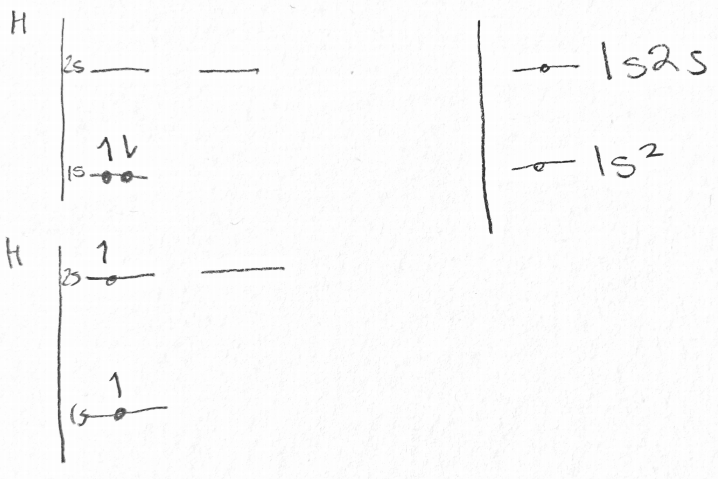
\includegraphics[width=0.7\linewidth]{hw4_1}
		
		
		\item \begin{enumerate}
			\item Assuming the form of (1) and ignoring mutual interaction, the potential term can be split into separate potentials for electron 1 and 2. This basically follows (6.1a) but with the last term equal to zero. \begin{align*}
				 H \psi_{1s2s} & = \hat{p_1}^2 \psi_{1s2s} + \hat{p_2}^2 \psi_{1s2s} + E_\mathrm{pot}\psi_{1s2s} \\
				& = \left(\hat{p_1}^2 + E_\mathrm{pot} \right)\psi_{1s}
				+ \left(\hat{p_2}^2 + E_\mathrm{pot} \right)\psi_{2s} \\
				& = H_1 + H_2
			\end{align*}
		
			\item There is not a way to distinguish these two wavefunctions, presumably because they are degenerate and would have equal energies and since the electrons are indistinguishable.
		\end{enumerate}
		
		\item Both (1) and (2) \underline{do not} abide by the Pauli principle. For (1), if we swap the electrons, we are left with $\psi_{2s}(\bvec{r}_1)\psi{1s}(\bvec{r}_2)$. For (2), it's the same thing but you would get back (1) after swapping the electrons.
		
		But (3) does abide by the Pauli principle. Swapping the electrons results in \begin{align*}
			\psi_{2s}(\bvec{r}_1) \psi_{1s}(\bvec{r}_2) - \psi_{1s}(\bvec{r}_1)\psi_{2s}(\bvec{r}_2) & = -\Psi_{1s2s}(\bvec{r}_2, \bvec{r}_1)
		\end{align*}
		...which is just the opposite of the original wavefunction.
		
		
		\item If they're both in $\psi_{1s}$, it would just be zero \begin{align*}
			\psi_{1s} \psi_{1s} - \psi_{1s} \psi_{1s} = 0
		\end{align*}
		This is the Pauli exclusion principle. 
		
		\item From (3), if both are now in the $1s$ state and we make electron 1 spin up, and electron 2 spin down, \begin{align*}
			\Psi_{1s^2}(1, 2) & = \psi_{1s}(1) \psi_{1s}(2) \ket{\uparrow} \ket{\downarrow} - \psi_{1s}(1) \psi_{1s}(2) \ket{\downarrow} \ket{\uparrow} \\
			& = \left( \psi_{1s}(1) \psi_{1s}(2)  - \psi_{1s}(1) \psi_{1s}(2)\right) \left(\ket{\uparrow \downarrow} - \ket{\downarrow \uparrow}\right) 
		\end{align*}
		It is Pauli approved. The spatial function is symmetric but the spinfunction is antisymmetric.
		
		\item  From (3), if we make electron 1 spin up, and electron 2 spin down, \begin{align*}
			\Psi_{1s2s}(1, 2) & = \psi_{1s}(1) \psi_{2s}(2) \ket{\uparrow} \ket{\downarrow} - \psi_{2s}(1) \psi_{1s}(2) \ket{\downarrow} \ket{\uparrow} \\
			& = \left( \psi_{1s}(1) \psi_{2s}(2)  - \psi_{2s}(1) \psi_{1s}(2)\right) \left(\ket{\uparrow \downarrow} - \ket{\downarrow \uparrow}\right) 
		\end{align*}
		\begin{enumerate}
			\item It is not Pauli approved. 
			\item Either the spatial function or spin function must be made symmetric: \begin{align*}
				\text{Case A: \quad } & \left( \psi_{1s}(1) \psi_{2s}(2)  + \psi_{2s}(1) \psi_{1s}(2)\right) \left(\ket{\uparrow \downarrow} - \ket{\downarrow \uparrow}\right) \\
				\text{Case B: \quad } & \left( \psi_{1s}(1) \psi_{2s}(2)  - \psi_{2s}(1) \psi_{1s}(2)\right) \left(\ket{\uparrow \downarrow} + \ket{\downarrow \uparrow}\right) 
			\end{align*}
			
		\end{enumerate}
	
		\item \begin{enumerate}
			\item The spatial function must be antisymmetric, since the spin function is now symmetric. So Case B.
			\item Case B.
		\end{enumerate}
	
		\item Yes, since it has multiplicity of $3$. The $m_s$ values are $-1, 0, 1$, which is consistent with $S=1$.
		
		\item Yes, since now it's multiplicity of $1$. The $m_s$ value is just $0$, since one electron is spin up, the other is spin down.
		
		\item \begin{enumerate}
			\item The triplet state. If $r_1 = r_2$, the antisymmetric spatial function would be zero.
			
			\item Yes, both figures show the triplet states lower in energy to their singlet state counterparts.
		\end{enumerate}
	\end{enumerate}
\end{document}